\begin{figure*}
%\vspace{-1em}
\centering
%\includegraphics[width=0.99\linewidth, trim={10cm 0 0 0},clip]{../yellowfin_iclr2018/manuscript_for_revision/experiment_results/resnet/mom_dynamic_3_annotated.pdf}
\includegraphics[width=0.99\linewidth]{../yellowfin_iclr2018/manuscript_for_revision/experiment_results/resnet/mom_dynamic_3_annotated.pdf}
	\vspace{-0.5em}
	\caption{
	When running \tuner, total momentum $\hat{\mu}_t$ equals algorithmic value in synchronous settings (left); $\hat{\mu}_t$ is greater than algorithmic value on 16 asynchronous workers (middle).
	\Asynctuner automatically lowers algorithmic momentum and brings total momentum to match the target value (right).
%Red dots are measured $\hat{\mu}_t$ at every step with red line as its running average.
	Red dots are total momentum estimates, $\hat{\mu}_T$, at each iteration. 
The solid red line is a running average of $\hat{\mu}_T$.
%	When running \tuner, total momentum $\hat{\mu}_t$ is greater than algorithmic value on 16 asynchronous workers (left).
%	\Asynctuner automatically lowers algorithmic momentum and matches total momentum to the target value (right).
%%Red dots are measured $\hat{\mu}_t$ at every step with red line as its running average.
%	Red dots are total momentum estimates, $\hat{\mu}_T$, at each iteration. 
%    The solid red line is a running average of $\hat{\mu}_T$.	
	}
	\label{fig:we-can-measure}
%\vspace{-0.35em}
\end{figure*}

\section{\Asynctuner}
\label{sec:async_tuner}

Asynchrony is a parallelization technique that avoids synchronization barriers \citep{recht2011hogwild}. 
In this section, we propose a {\em closed momentum loop} variant of \tuner to accelerate convergence in asynchronous training. 
%To handle the momentum dynamics of asynchronous parallelism, we propose a {\em closed momentum loop} variant of \tuner.
After some preliminaries, we show the mechanism of the extension: 
it measures the dynamics on a running system and controls momentum with a negative feedback loop.
\paragraph{Preliminaries}
%Asynchrony is a popular parallelization technique \citep{recht2011hogwild} that avoids synchronization barriers.
When training on $M$ asynchronous workers, staleness (the number of model updates between a worker's read and write operations) is on average $\tau=M-1$,
i.e., the gradient in the SGD update is delayed by $\tau$ iterations as $\nabla f_{S_{t - \tau}}(x_{t - \tau} )$.
Asynchrony yields faster steps, but can
increase the number of iterations to achieve the same solution,
a tradeoff between hardware and statistical 
efficiency~\citep{DBLP:journals/pvldb/ZhangR14}.
\citet{mitliagkas2016asynchrony} interpret asynchrony as added momentum dynamics.
Experiments in \citet{hadjis2016omnivore} support this finding, and demonstrate that reducing algorithmic momentum can compensate for asynchrony-induced momentum
and significantly reduce the number of iterations for convergence.
Motivated by that result, we use the model
in~\eqref{equ:exp_async_update_app}, where the total momentum, $\mu_T$, includes both asynchrony-induced and algorithmic  momentum, $\mu$, in~\eqref{eqn:momentum_gd}.
\begin{equation}
	\mathbb{E}[ x_{t+1} - x_t ] 
	= \mu_T \mathbb{E}[x_t - x_{t-1}] - \alpha \mathbb{E}\nabla f(x_{t})
\label{equ:exp_async_update_app}
\end{equation}
We will use this expression to design an estimator for the value of total momentum, $\hat{\mu}_T$.
This estimator is a basic building block of \asynctuner, that {\em removes the need to manually compensate for the effects of asynchrony}.



\paragraph{Measuring the momentum dynamics}
\Asynctuner estimates total momentum $\mu_{T}$ on a running system and uses a negative feedback loop to adjust algorithmic momentum accordingly.
Equation~\eqref{equ:exp_async_update} gives an estimate of $\hat{\mu}_T$ on a system with staleness $\tau$, based on \eqref{equ:exp_async_update}.
\begin{align}
\hat{\mu}_T
					= \mathop{\mathsf{median}}\left(
							\frac{x_{t - \tau} - x_{t - \tau-1} + \alpha \nabla_{S_{t-\tau -1}} f(x_{t - \tau - 1} )}
							{x_{t - \tau-1} - x_{t - \tau-2}}
					\right)
\label{eqn:momentum_measurement}
\end{align}
We use $\tau$-stale model values to match the staleness of the gradient,  and perform all operations in an elementwise fashion. 
This way we get a total momentum measurement from each variable; 
the median combines them into a more robust estimate.

\paragraph{Closing the asynchrony loop}
Given a reliable measurement of $\mu_{T}$, 
we can use it to adjust the value of algorithmic momentum so that the total momentum matches the \emph{target momentum} as decided by \tuner in Algorithm~\ref{alg:basic-algo}.
\Asynctuner in Algorithm~\ref{alg:async-algo} %(in Appendix~\ref{sec:async_yf}) 
uses a simple negative feedback loop to achieve the adjustment.
%Figure~\ref{fig:we-can-measure} demonstrates that under asynchrony the measured total momentum is strictly higher than the algorithmic momentum (middle plot), as expected from theory;
%closing the feedback loop (right plot) leads to total momentum matching the target momentum.
%Closing the loop, as we will see, improves performance significantly.
%Note for asynchronous-parallel training, as the estimates and parameter tuning is unstable in the beginning when there are only a small number of iterations, we use initial learning $\frac{1}{\tau + 1}$ instead of $1.0$ to prevent overflow in the beginning. 

%\begin{algorithm}[H]
%	\caption{\Asynctuner}
%	\begin{algorithmic}[1]
%%	\State Input: $\mu\gets0$, $\alpha \gets \frac{1}{\tau + 1}$, $\gamma\gets0.01, \tau$ (staleness)
%	\State Input: $\mu\gets0$, $\alpha \gets 0.0001$, $\gamma\gets0.01, \tau$ (staleness)
%	\For { $t\gets1$ to $T$}
%	\State $x_t\!\gets\!x_{t - 1} + \mu (x_{t - 1} - x_{t - 2} ) - \alpha \nabla_{S_t} f(x_{t - \tau - 1} )$
%	\State $\mu^*,\alpha \gets \Call{\tuner}{\nabla_{S_t} f(x_{t - \tau - 1} ), \beta}$ %(get momentum from the dynamic range)
%	\State $\hat{\mu_T} 
%					\gets \mathop{\mathsf{median}}\left(
%							\frac{x_{t - \tau} - x_{t - \tau-1} + \alpha \nabla_{S_{t-\tau-1}} f(x_{t - \tau - 1} )}
%							{x_{t - \tau-1} - x_{t - \tau-2}}
%					\right)$ \Comment{Measuring total momentum}
%	\State $\mu \leftarrow \mu + \gamma \cdot (\mu^* - \hat{\mu_T})$ \Comment{Closing the loop}
%	\EndFor
%\end{algorithmic}
%\label{alg:async-algo}
%\end{algorithm}




%In Section~\ref{sec:async_tuner}, we briefly discuss the mechanism of our designed \Asynctuner in asynchronous-parallel setting. In this appendix, we expand the details in total momentum estimator, $\hat{\mu_T}$, and present the full \Asynctuner in Algorithm~\ref{alg:async-algo} with extensive discussion.
%\paragraph{Measuring the momentum dynamics}
%Remember, we use the formula in~\eqref{equ:exp_async_update_app} to model the momentum dynamics in asynchronous-parallel systems
%\Asynctuner estimates total momentum $\mu_{T}$ on a running system and uses a negative feedback loop to adjust algorithmic momentum accordingly.
%\begin{equation}
%	\mathbb{E}[ x_{t+1} - x_t ] 
%	= \mu_T \mathbb{E}[x_t - x_{t-1}] - \alpha \mathbb{E}\nabla f(x_{t})
%\label{equ:exp_async_update_app}
%\end{equation}
%Equation~\eqref{eqn:momentum_measurement_app} gives an estimate of $\hat{\mu_T}$ on a system with staleness $\tau$, based on \eqref{equ:exp_async_update_app}.
%\begin{align}
%\hat{\mu_T}
%					= \mathop{\mathsf{median}}\left(
%							\frac{x_{t - \tau} - x_{t - \tau-1} + \alpha \nabla_{S_{t-\tau -1}} f(x_{t - \tau - 1} )}
%							{x_{t - \tau-1} - x_{t - \tau-2}}
%					\right)
%\label{eqn:momentum_measurement_app}
%\end{align}
%We use $\tau$-stale model values to match the staleness of the gradient,  and perform all operations in an elementwise fashion. 
%This way we get a total momentum measurement from each variable; 
%the median combines them into a more robust estimate.
%
%%\label{subsec:closed_loop_YF}
%%\begin{figure}
%%\centering
%%\includegraphics[width=0.95\linewidth]{experiment_results/resnet/mom_dynamic_3_annotated.pdf}
%%	\caption{
%%	Momentum dynamics on CIFAR100 ResNet.
%%	Running \tuner, total momentum is equal to algorithmic momentum in a synchronous setting (left). Total momentum is greater than algorithmic momentum on 16 asynchronous workers, due to asynchrony-induced momentum (middle).
%%	Using the momentum feedback mechanism of \asynctuner, lowers algorithmic momentum and brings total momentum to match the target value on 16 asynchronous workers (right).
%%	Red dots are individual total momentum estimates, $\hat{\mu}_T$, at each iteration. 
%%The solid red line is a running average of those estimates.	
%%	}
%%	\label{fig:we-can-measure}
%%\end{figure}
%
%\paragraph{Closing the asynchrony loop}
%Given a reliable measurement of $\mu_{T}$, 
%we can use it to adjust the value of algorithmic momentum so that the total momentum matches the \emph{target momentum} as decided by \tuner in Algorithm~\ref{alg:basic-algo}.
%\Asynctuner in Algorithm~\ref{alg:async-algo} %(in Appendix~\ref{sec:async_yf}) 
%uses a simple negative feedback loop to achieve the adjustment.
%%Figure~\ref{fig:we-can-measure} demonstrates that under asynchrony the measured total momentum is strictly higher than the algorithmic momentum (middle plot), as expected from theory;
%%closing the feedback loop (right plot) leads to total momentum matching the target momentum.
%%Closing the loop, as we will see, improves performance significantly.
%%%Note for asynchronous-parallel training, as the estimates and parameter tuning is unstable in the beginning when there are only a small number of iterations, we use initial learning $\frac{1}{\tau + 1}$ instead of $1.0$ to prevent overflow in the beginning. 
%%
%%%\begin{algorithm}[H]
%%%	\caption{\Asynctuner}
%%%	\begin{algorithmic}[1]
%%%%	\State Input: $\mu\gets0$, $\alpha \gets \frac{1}{\tau + 1}$, $\gamma\gets0.01, \tau$ (staleness)
%%%	\State Input: $\mu\gets0$, $\alpha \gets 0.0001$, $\gamma\gets0.01, \tau$ (staleness)
%%%	\For { $t\gets1$ to $T$}
%%%	\State $x_t\!\gets\!x_{t - 1} + \mu (x_{t - 1} - x_{t - 2} ) - \alpha \nabla_{S_t} f(x_{t - \tau - 1} )$
%%%	\State $\mu^*,\alpha \gets \Call{\tuner}{\nabla_{S_t} f(x_{t - \tau - 1} ), \beta}$ %(get momentum from the dynamic range)
%%%	\State $\hat{\mu_T} 
%%%					\gets \mathop{\mathsf{median}}\left(
%%%							\frac{x_{t - \tau} - x_{t - \tau-1} + \alpha \nabla_{S_{t-\tau-1}} f(x_{t - \tau - 1} )}
%%%							{x_{t - \tau-1} - x_{t - \tau-2}}
%%%					\right)$ \Comment{Measuring total momentum}
%%%	\State $\mu \leftarrow \mu + \gamma \cdot (\mu^* - \hat{\mu_T})$ \Comment{Closing the loop}
%%%	\EndFor
%%%\end{algorithmic}
%%%\label{alg:async-algo}
%%%\end{algorithm}
%%
%
%
%




\begin{algorithm}[h]
	\caption{\Asynctuner}
	\begin{algorithmic}[1]
%	\State Input: $\mu\gets0$, $\alpha \gets \frac{1}{\tau + 1}$, $\gamma\gets0.01, \tau$ (staleness)
	\State Input: $\mu\gets0$, $\alpha \gets 0.0001$, $\gamma\gets0.01, \tau$ (staleness)
	\For { $t\gets1$ to $T$}
	\State $x_t\!\gets\!x_{t - 1} + \mu (x_{t - 1} - x_{t - 2} ) - \alpha \nabla_{S_t} f(x_{t - \tau - 1} )$
	\State $\mu^*,\alpha \gets \Call{\tuner}{\nabla_{S_t} f(x_{t - \tau - 1} ), \beta}$ %(get momentum from the dynamic range)
	\State $\hat{\mu_T} 
					\gets \mathop{\mathsf{median}}\left(
							\frac{x_{t - \tau} - x_{t - \tau-1} + \alpha \nabla_{S_{t-\tau-1}} f(x_{t - \tau - 1} )}
							{x_{t - \tau-1} - x_{t - \tau-2}}
					\right)$ \Comment{Measuring total momentum}
	\State $\mu \leftarrow \mu + \gamma \cdot (\mu^* - \hat{\mu_T})$ \Comment{Closing the loop}
	\EndFor
\end{algorithmic}
\label{alg:async-algo}
\end{algorithm}


%%%%%%%%%%%%%%%%% latest backup version %%%%%%%%%%%%%%%%%%%%%%%%%%%%%%%%%%%%
%Asynchrony is a parallelization technique that avoids synchronization barriers \citep{recht2011hogwild}. 
%%In this section, we propose a {\em closed momentum loop} variant of \tuner to accelerate convergence in asynchronous training. 
%%To handle the momentum dynamics of asynchronous parallelism, we propose a {\em closed momentum loop} variant of \tuner.
%%After some preliminaries, we show the mechanism of the extension: 
%%it measures the dynamics on a running system and controls momentum with a negative feedback loop.
%%\paragraph{Preliminaries}
%%Asynchrony is a popular parallelization technique \citep{recht2011hogwild} that avoids synchronization barriers.
%%When training on $M$ asynchronous workers, staleness (the number of model updates between a worker's read and write operations) is on average $\tau=M-1$,
%%i.e., the gradient in the SGD update is delayed by $\tau$ iterations as $\nabla f_{S_{t - \tau}}(x_{t - \tau} )$.
%%It yields faster steps, but can
%%increase the number of iterations needed,
%%a tradeoff between hardware and statistical 
%%efficiency~\citep{DBLP:journals/pvldb/ZhangR14}.
%It yields better hardware efficiency, i.e. faster steps, but can
%increase the number of iterations to a given metric, i.e. statistical efficiency, as a tradeoff~\citep{DBLP:journals/pvldb/ZhangR14}.
%%a tradeoff between hardware and statistical 
%%efficiency~\citep{DBLP:journals/pvldb/ZhangR14}.
%%In this section, we propose a {\em closed momentum loop} variant of \tuner to reduce the number of iterations it needs to converge in asynchronous training. 
%%In this section, we propose a {\em closed momentum loop} variant of \tuner to reduce the number of iterations for convergence in asynchronous training.
%%\paragraph{\Asynctuner}
%\citet{mitliagkas2016asynchrony} interpret asynchrony as added momentum dynamics.
%%It is empirically supported in \citet{hadjis2016omnivore} that manually reducing algorithmic momentum can compensate for asynchrony-induced momentum
%%and significantly reduce the number of iterations to converge.
%We design \asynctuner, a variant of \tuner to automatically control algorithmic momentum, compensate for asynchrony and accelerate convergence.
%We use the formula in~\eqref{equ:exp_async_update} to model the dynamics in the system, where the total momentum, $\mu_T$, includes both asynchrony-induced and algorithmic  momentum, $\mu$, in~\eqref{eqn:momentum_gd}.
%\begin{equation}
%	\mathbb{E}[ x_{t+1} - x_t ] 
%	= \mu_T \mathbb{E}[x_t - x_{t-1}] - \alpha \mathbb{E}\nabla f(x_{t})
%\label{equ:exp_async_update}
%\end{equation}
%We first use~\eqref{equ:exp_async_update} to design an robust estimator $\hat{\mu}_T$ for the value of total momentum at every iteration.
%%This estimator is a basic building block of \asynctuner, that {\em removes the need to manually compensate for the effects of asynchrony}. 
%Then we use a simple negative feedback control loop to adjust the value of algorithmic momentum so that $\hat{\mu}_T$ matches the \emph{target momentum} decided by \tuner in Algorithm~\ref{alg:basic-algo}. 
%%We refer to Appendix~\ref{sec:async_app} for details on estimator $\hat{\mu}_T$ and \Asynctuner in Algorithm~\ref{alg:async-algo}.
%%\Asynctuner in Algorithm~\ref{alg:async-algo} (in Appendix~\ref{sec:async_app}) %(in Appendix~\ref{sec:async_yf}) 
%%uses a simple negative feedback loop to achieve the adjustment.
%In Figure~\ref{fig:we-can-measure}, 
%we demonstrate momentum dynamics in an asynchronous training system. 
%As directly using the target value as algorithmic momentum, \tuner (middle) presents total momentum $\hat{\mu}_T$ strictly larger than the target momentum, due to asynchrony-induced momentum. \Asynctuner (right) automatically brings down algorithmic momentum, match measured total momentum $\hat{\mu}_T$ to target value and, as we will see, speeds up convergence comparing to \tuner. We refer to Appendix~\ref{sec:async_app} for details on estimator $\hat{\mu}_T$ and \Asynctuner in Algorithm~\ref{alg:async-algo}.
%%
%%so that visually demonstrates the mechanism of \Asynctuner in handling the momentum dynamics under asynchrony. In asynchronous-parallel setting, the measured total momentum is strictly higher than the algorithmic momentum (middle plot), as expected from theory.
%%Closing the feedback loop (right plot) leads to total momentum matching the target momentum and, as we will see, improves performance significantly.
%
%%\begin{figure*}
%%%\vspace{-2.5em}
%%\centering
%%\includegraphics[width=\linewidth]{experiment_results/resnet/mom_dynamic_3_annotated.pdf}
%%	\caption{
%%	When running \tuner, total momentum $\hat{\mu}_t$ equals algorithmic value in synchronous settings (left); $\hat{\mu}_t$ is greater than algorithmic value on 16 asynchronous workers (middle).
%%	\Asynctuner automatically lowers algorithmic momentum and brings total momentum to match the target value (right).
%%Red dots are measured $\hat{\mu}_t$ at every step with red line as its running average.
%%%	Red dots are total momentum estimates, $\hat{\mu}_T$, at each iteration. 
%%%The solid red line is a running average of $\hat{\mu}_T$.	
%%	}
%%	\vspace{-0.25em}
%%	\label{fig:we-can-measure}
%%\end{figure*}


%%%%%%%%%%%%%%%%%%%%%% latest backup versions %%%%%%%%%%%%%%%%%%%%%%%%%%%%%%%%%%%%%%%%%
%%\begin{figure}
%%\centering
%%\includegraphics[width=0.95\linewidth]{experiment_results/resnet/mom_dynamic_3_annotated.pdf}
%%	\caption{
%%%	Momentum dynamics on CIFAR100 ResNet.
%%	Running \tuner on a ResNet, total momentum equals algorithmic value in a synchronous setting (left). Total momentum is greater than algorithmic value on 16 asynchronous workers, due to asynchrony-induced momentum (middle).
%%	\asynctuner automatically lowers algorithmic momentum and brings total momentum to match the target value (right).
%%	Red dots are total momentum estimates, $\hat{\mu}_T$, at each iteration. 
%%The solid red line is a running average of $\hat{\mu}_T$.	
%%	}
%%	\label{fig:we-can-measure}
%%\end{figure}
%Asynchrony is a parallelization technique that avoids synchronization barriers \citep{recht2011hogwild}. 
%%In this section, we propose a {\em closed momentum loop} variant of \tuner to accelerate convergence in asynchronous training. 
%%To handle the momentum dynamics of asynchronous parallelism, we propose a {\em closed momentum loop} variant of \tuner.
%%After some preliminaries, we show the mechanism of the extension: 
%%it measures the dynamics on a running system and controls momentum with a negative feedback loop.
%%\paragraph{Preliminaries}
%%Asynchrony is a popular parallelization technique \citep{recht2011hogwild} that avoids synchronization barriers.
%%When training on $M$ asynchronous workers, staleness (the number of model updates between a worker's read and write operations) is on average $\tau=M-1$,
%%i.e., the gradient in the SGD update is delayed by $\tau$ iterations as $\nabla f_{S_{t - \tau}}(x_{t - \tau} )$.
%%It yields faster steps, but can
%%increase the number of iterations needed,
%%a tradeoff between hardware and statistical 
%%efficiency~\citep{DBLP:journals/pvldb/ZhangR14}.
%It yields better hardware efficiency, i.e. faster steps, but can
%increase the number of iterations to a given metric, i.e. statistical efficiency, as a tradeoff~\citep{DBLP:journals/pvldb/ZhangR14}.
%%a tradeoff between hardware and statistical 
%%efficiency~\citep{DBLP:journals/pvldb/ZhangR14}.
%%In this section, we propose a {\em closed momentum loop} variant of \tuner to reduce the number of iterations it needs to converge in asynchronous training. 
%%In this section, we propose a {\em closed momentum loop} variant of \tuner to reduce the number of iterations for convergence in asynchronous training.
%%\paragraph{\Asynctuner}
%\citet{mitliagkas2016asynchrony} interpret asynchrony as added momentum dynamics.
%%It is empirically supported in \citet{hadjis2016omnivore} that manually reducing algorithmic momentum can compensate for asynchrony-induced momentum
%%and significantly reduce the number of iterations to converge.
%We design a {\em closed momentum loop} variant of \tuner to control algorithmic momentum, compensate for asynchrony and accelerate convergence.
%We use the formula in~\eqref{equ:exp_async_update} to model the dynamics in the system, where the total momentum, $\mu_T$, includes both asynchrony-induced and algorithmic  momentum, $\mu$, in~\eqref{eqn:momentum_gd}.
%\begin{equation}
%	\mathbb{E}[ x_{t+1} - x_t ] 
%	= \mu_T \mathbb{E}[x_t - x_{t-1}] - \alpha \mathbb{E}\nabla f(x_{t})
%\label{equ:exp_async_update}
%\end{equation}
%We first use this expression to design an robust estimator $\hat{\mu}_T$ for the value of total momentum.
%%This estimator is a basic building block of \asynctuner, that {\em removes the need to manually compensate for the effects of asynchrony}.
%Given $\hat{\mu}_T$,  
%we use it to adjust the value of algorithmic momentum so that the total momentum matches the \emph{target momentum} decided by \tuner in Algorithm~\ref{alg:basic-algo}. Specifically, we %\asynctuner  %(in Appendix~\ref{sec:async_yf}) 
%uses a simple negative feedback loop to achieve the adjustment. We refer to Appendix~\ref{sec:async_app} for details on estimator $\hat{\mu}_T$ and \Asynctuner in Algorithm~\ref{alg:async-algo}.
%%\Asynctuner in Algorithm~\ref{alg:async-algo} (in Appendix~\ref{sec:async_app}) %(in Appendix~\ref{sec:async_yf}) 
%%uses a simple negative feedback loop to achieve the adjustment.
%Figure~\ref{fig:we-can-measure} visually demonstrates the mechanism of \Asynctuner in handling the momentum dynamics under asynchrony. In asynchronous-parallel setting, the measured total momentum is strictly higher than the algorithmic momentum (middle plot), as expected from theory.
%Closing the feedback loop (right plot) leads to total momentum matching the target momentum and, as we will see, improves performance significantly.
%
%\begin{figure}
%\centering
%\includegraphics[width=0.95\linewidth]{experiment_results/resnet/mom_dynamic_3_annotated.pdf}
%	\caption{
%%	Momentum dynamics on CIFAR100 ResNet.
%	Running \tuner on a ResNet, total momentum equals algorithmic value in a synchronous setting (left). Total momentum is greater than algorithmic value on 16 asynchronous workers, due to asynchrony-induced momentum (middle).
%	\asynctuner automatically lowers algorithmic momentum and brings total momentum to match the target value (right).
%	Red dots are total momentum estimates, $\hat{\mu}_T$, at each iteration. 
%The solid red line is a running average of $\hat{\mu}_T$.	
%	}
%	\label{fig:we-can-measure}
%\end{figure}
%

%%%%%%%%%%%%%%%%%%%%%% below are old backup versions %%%%%%%%%%%%%%%%%%%%%%%%%%%%%%%%%%

%\paragraph{Measuring the momentum dynamics}
%\Asynctuner estimates total momentum $\mu_{T}$ on a running system and uses a negative feedback loop to adjust algorithmic momentum accordingly.
%Equation~\eqref{equ:exp_async_update} gives an estimate of $\hat{\mu_T}$ on a system with staleness $\tau$, based on \eqref{equ:exp_async_update}.
%\begin{align}
%\hat{\mu_T}
%					= \mathop{\mathsf{median}}\left(
%							\frac{x_{t - \tau} - x_{t - \tau-1} + \alpha \nabla_{S_{t-\tau -1}} f(x_{t - \tau - 1} )}
%							{x_{t - \tau-1} - x_{t - \tau-2}}
%					\right)
%\label{eqn:momentum_measurement}
%\end{align}
%We use $\tau$-stale model values to match the staleness of the gradient,  and perform all operations in an elementwise fashion. 
%This way we get a total momentum measurement from each variable; 
%the median combines them into a more robust estimate.

%\label{subsec:closed_loop_YF}
%\begin{figure}
%\centering
%\includegraphics[width=0.95\linewidth]{experiment_results/resnet/mom_dynamic_3_annotated.pdf}
%	\caption{
%	Momentum dynamics on CIFAR100 ResNet.
%	Running \tuner, total momentum is equal to algorithmic momentum in a synchronous setting (left). Total momentum is greater than algorithmic momentum on 16 asynchronous workers, due to asynchrony-induced momentum (middle).
%	Additionally applying the momentum feedback loop of \asynctuner, lowers algorithmic momentum and matches total momentum to target value (right).
%	Red dots are individual total momentum estimates, $\hat{\mu}_T$, at each iteration, with
%the solid red line as its running average.	
%	}
%	\label{fig:we-can-measure}
%\end{figure}

%\paragraph{Closing the asynchrony loop}
%Given a reliable measurement of $\mu_{T}$, 
%we can use it to adjust the value of algorithmic momentum so that the total momentum matches the \emph{target momentum} as decided by \tuner in Algorithm~\ref{alg:basic-algo}.
%\Asynctuner in Algorithm~\ref{alg:async-algo} (in Appendix~\ref{sec:async_app}) %(in Appendix~\ref{sec:async_yf}) 
%uses a simple negative feedback loop to achieve the adjustment.
%Figure~\ref{fig:we-can-measure} demonstrates that under asynchrony the measured total momentum is strictly higher than the algorithmic momentum (middle plot), as expected from theory;
%closing the feedback loop (right plot) leads to total momentum matching the target momentum.
%Closing the loop, as we will see, improves performance significantly.
%





%To handle the momentum dynamics of asynchronous parallelism, we propose a {\em closed momentum loop} variant of \tuner.
%After some preliminaries, we show the mechanism of the extension: 
%it measures the dynamics on a running system and controls momentum with a negative feedback loop.
%\paragraph{Preliminaries}
%Asynchrony is a popular parallelization technique \citep{recht2011hogwild} that avoids synchronization barriers.
%When training on $M$ asynchronous workers, staleness (the number of model updates between a worker's read and write operations) is on average $\tau=M-1$,
%i.e., the gradient in the SGD update is delayed by $\tau$ iterations as $\nabla f_{S_{t - \tau}}(x_{t - \tau} )$.
%Asynchrony yields faster steps, but can
%increase the number of iterations to achieve the same solution,
%a tradeoff between hardware and statistical 
%efficiency~\citep{DBLP:journals/pvldb/ZhangR14}.
%\citet{mitliagkas2016asynchrony} interpret asynchrony as added momentum dynamics.
%Experiments in \citet{hadjis2016omnivore} support this finding, and demonstrate that reducing algorithmic momentum can compensate for asynchrony-induced momentum
%and significantly reduce the number of iterations for convergence.
%Motivated by that result, we use the model
%in~\eqref{equ:exp_async_update}, where the total momentum, $\mu_T$, includes both asynchrony-induced and algorithmic  momentum, $\mu$, in~\eqref{eqn:momentum_gd}.
%\begin{equation}
%	\mathbb{E}[ x_{t+1} - x_t ] 
%	= \mu_T \mathbb{E}[x_t - x_{t-1}] - \alpha \mathbb{E}\nabla f(x_{t})
%\label{equ:exp_async_update}
%\end{equation}
%We will use this expression to design an estimator for the value of total momentum, $\hat{\mu_T}$.
%This estimator is a basic building block of \asynctuner, that {\em removes the need to manually compensate for the effects of asynchrony}.
%
%
%
%\paragraph{Measuring the momentum dynamics}
%\Asynctuner estimates total momentum $\mu_{T}$ on a running system and uses a negative feedback loop to adjust algorithmic momentum accordingly.
%Equation~\eqref{equ:exp_async_update} gives an estimate of $\hat{\mu_T}$ on a system with staleness $\tau$, based on \eqref{equ:exp_async_update}.
%\begin{align}
%\hat{\mu_T}
%					= \mathop{\mathsf{median}}\left(
%							\frac{x_{t - \tau} - x_{t - \tau-1} + \alpha \nabla_{S_{t-\tau -1}} f(x_{t - \tau - 1} )}
%							{x_{t - \tau-1} - x_{t - \tau-2}}
%					\right)
%\label{eqn:momentum_measurement}
%\end{align}
%We use $\tau$-stale model values to match the staleness of the gradient,  and perform all operations in an elementwise fashion. 
%This way we get a total momentum measurement from each variable; 
%the median combines them into a more robust estimate.
%
%\label{subsec:closed_loop_YF}
%\begin{figure}
%\centering
%\includegraphics[width=0.95\linewidth]{experiment_results/resnet/mom_dynamic_3_annotated.pdf}
%	\caption{
%	Momentum dynamics on CIFAR100 ResNet.
%	Running \tuner, total momentum is equal to algorithmic momentum in a synchronous setting (left). Total momentum is greater than algorithmic momentum on 16 asynchronous workers, due to asynchrony-induced momentum (middle).
%	Using the momentum feedback mechanism of \asynctuner, lowers algorithmic momentum and brings total momentum to match the target value on 16 asynchronous workers (right).
%	Red dots are individual total momentum estimates, $\hat{\mu}_T$, at each iteration. 
%The solid red line is a running average of those estimates.	
%	}
%	\label{fig:we-can-measure}
%\end{figure}
%
%\paragraph{Closing the asynchrony loop}
%Given a reliable measurement of $\mu_{T}$, 
%we can use it to adjust the value of algorithmic momentum so that the total momentum matches the \emph{target momentum} as decided by \tuner in Algorithm~\ref{alg:basic-algo}.
%\Asynctuner in Algorithm~\ref{alg:async-algo} (in Appendix~\ref{sec:async_app}) %(in Appendix~\ref{sec:async_yf}) 
%uses a simple negative feedback loop to achieve the adjustment.
%Figure~\ref{fig:we-can-measure} demonstrates that under asynchrony the measured total momentum is strictly higher than the algorithmic momentum (middle plot), as expected from theory;
%closing the feedback loop (right plot) leads to total momentum matching the target momentum.
%Closing the loop, as we will see, improves performance significantly.
%%Note for asynchronous-parallel training, as the estimates and parameter tuning is unstable in the beginning when there are only a small number of iterations, we use initial learning $\frac{1}{\tau + 1}$ instead of $1.0$ to prevent overflow in the beginning. 
%
%%\begin{algorithm}[H]
%%	\caption{\Asynctuner}
%%	\begin{algorithmic}[1]
%%%	\State Input: $\mu\gets0$, $\alpha \gets \frac{1}{\tau + 1}$, $\gamma\gets0.01, \tau$ (staleness)
%%	\State Input: $\mu\gets0$, $\alpha \gets 0.0001$, $\gamma\gets0.01, \tau$ (staleness)
%%	\For { $t\gets1$ to $T$}
%%	\State $x_t\!\gets\!x_{t - 1} + \mu (x_{t - 1} - x_{t - 2} ) - \alpha \nabla_{S_t} f(x_{t - \tau - 1} )$
%%	\State $\mu^*,\alpha \gets \Call{\tuner}{\nabla_{S_t} f(x_{t - \tau - 1} ), \beta}$ %(get momentum from the dynamic range)
%%	\State $\hat{\mu_T} 
%%					\gets \mathop{\mathsf{median}}\left(
%%							\frac{x_{t - \tau} - x_{t - \tau-1} + \alpha \nabla_{S_{t-\tau-1}} f(x_{t - \tau - 1} )}
%%							{x_{t - \tau-1} - x_{t - \tau-2}}
%%					\right)$ \Comment{Measuring total momentum}
%%	\State $\mu \leftarrow \mu + \gamma \cdot (\mu^* - \hat{\mu_T})$ \Comment{Closing the loop}
%%	\EndFor
%%\end{algorithmic}
%%\label{alg:async-algo}
%%\end{algorithm}
%
